\chapter{実装}
\label{implementation}

本章では提案手法の実装について述べる.

\section{実装環境}
\label{implementation:environment}

本節では,本研究で構築した実装環境について概説する.

\subsection{ハードウェアおよびソフトウェア}
\label{implementation:environment:resouces}

本研究で使用したハードウェアおよびソフトウェアとそのバージョンを以下に示す.

\begin{table}[htb]
  \begin{center}
    \caption{使用したハードウェアおよびソフトウェア}
    \begin{tabular}{|l|l|} \hline
      ハードウェア/ソフトウェア & 機種/バージョン \\ \hline
      Server & FUJITSU PRIMERGY S6 \\ \hline
      VMWare ESXi & 6.5 \\ \hline
      VyOS & 1.2.1 \\ \hline
      OpenVPN & 2.3.4 \\ \hline
      Ubuntu & 18.04 \\ \hline
      kubeadm & 1.16.3 \\ \hline
      kubelet & 1.16.3 \\ \hline
      kubectl & 1.16.3 \\ \hline
    \end{tabular}
  \end{center}
\end{table}

\subsection{物理サーバの準備}
\label{implementation:esxi}

本研究では、実装において複数のセグメントおよびKubernetesクラスタの構築に複数のサーバが必要であったため、それらを仮想的に作成できるVMWare ESXi(以下、ESXi)を導入した。
使用したのは、ESXi6.5だ。
ESXiはホストOSを必要とせず、直接ハードウェアにインストールさせて動作させるハイパーバイザー型であるため、まず初めにESXiインストーラの
ブータブルイメージをUSBメモリに書き込み、FUJITSUサーバにインストールした。
計二台のFUJITSUサーバにESXiをインストールし、それぞれ以下のIPアドレスを設定した。

\begin{table}[htb]
  \begin{center}
    \caption{ESXiのIPアドレス}
    \begin{tabular}{|l|l|} \hline
      名前 & IPアドレス \\ \hline
      1台目 & 10.4.0.13 \\ \hline
      2台目 & 10.4.0.14 \\ \hline
    \end{tabular}
  \end{center}
\end{table}

\subsection{ネットワーク構成}
\label{implementation:network-environment}

本研究で構築したネットワーク構成について説明する。

まず初めに、ESXiの仮想スイッチとVLANを用いて二つのESXiサーバ上に新たに計三つの論理セグメントを構築した。
Vlanによって論理的にセグメントを分割することで、お互いに通信不可能な環境とした。
以下に、Vlan IDと対応するアドレスプレフィックスを示す。
なお、10.4.0.0/16のアドレスプレフィックスはVlan ID 0に対応している。

\begin{table}[htb]
  \begin{center}
    \caption{Vlan IDと対応するアドレスプレフィックス}
    \begin{tabular}{|l|l|} \hline
      Vlan ID & アドレスプレフィックス \\ \hline
      0 & 10.4.0.0/16 \\ \hline
      10 & 192.168.10.0/24 \\ \hline
      20 & 192.168.20.0/24 \\ \hline
      30 & 192.168.30.0/24 \\ \hline
    \end{tabular}
  \end{center}
\end{table}

\subsection{VMの配置}

ネットワーク構築後、Kubernetesクラスタの構築に必要なサーバをVMとして立ち上げた。
それぞれのVMのOSにはUbuntu18.04を採用した。
以下に構築したサーバの詳細を示す。

\begin{landscape}
  \begin{table}[htb]
    \begin{center}
      \caption{設置したVMの詳細}
      \begin{tabular}{|l|l|l|l|l|} \hline
        名前 & ネットワークインターフェース名 & Vlan ID & IPアドレス & 役割 \\ \hline
        lb & ens160 & 10 & 192.168.10.253 & マスターノードのロードバランサー \\ \hline
        master01 & ens160 & 10 & 192.168.10.101 & マスターノード \\ \hline
        master02 & ens160 & 10 & 192.168.10.102 & マスターノード \\ \hline
        master03 & ens160 & 10 & 192.168.10.103 & マスターノード \\ \hline
        node01 & ens160 & 20 & 192.168.20.101 & ワーカーノード \\ \hline
        node02 & ens160 & 20 & 192.168.20.102 & ワーカーノード \\ \hline
        node03 & ens160 & 30 & 192.168.30.101 & ワーカーノード \\ \hline
        node04 & ens160 & 30 & 192.168.30.102 & ワーカーノード \\ \hline
      \end{tabular}
    \end{center}
  \end{table}
\end{landscape}

\subsection{ルーターの配置}

次に各拠点にOpenVPNの設定をするルーターを設置した。
ルーターのOSにはVyOS 1.2.1、OpenVPNはバージョン2.3.4を採用した。
以下にルーターのネットワーク情報を示す。

\begin{table}[htb]
  \begin{center}
    \caption{設置したルーターの詳細}
    \begin{tabular}{|l|l|l|l|l|} \hline
      名前 & ネットワークインターフェース名 & Vlan ID & IPアドレス \\ \hline
      vyos01 & eth0 & 0 & 10.4.0.90 \\ \hline
      vyos01 & eth1 & 10 & 192.168.10.1 \\ \hline
      vyos02 & eth0 & 0 & 10.4.0.91 \\ \hline
      vyos02 & eth1 & 20 & 192.168.20.1 \\ \hline
      vyos03 & eth0 & 0 & 10.4.0.92 \\ \hline
      vyos03 & eth1 & 30 & 192.168.30.1 \\ \hline
    \end{tabular}
  \end{center}
\end{table}

全てのルーターはお互いに疎通可能である。
さらに、各拠点に設置されたサーバと疎通できるようeth1のネットワークインターフェースには別のIPアドレスを設定した。
この時点での各サーバの疎通性は以下の通りである。

\begin{table}[htb]
  \begin{center}
    \caption{OpenVPN設定前の各サーバの疎通性}
    \begin{tabular}{|c|c|c|c|c|c|c|c|c|} \hline
      & lb & master01 & master02 & master03 & node01 & node02 & node03 & node04 \\ \hline
      lb & \ & ○ & ○ & ○ & × & × & × & × \\ \hline
      master01 & ○ & \ & ○ & ○ & × & × & × & × \\ \hline
      master02 & ○ & ○ & \ & ○ & × & × & × & × \\ \hline
      master03 & ○ & ○ & ○ & \ & × & × & × & × \\ \hline
      node01 & × & × & × & × & \ & ○ & × & × \\ \hline
      node02 & × & × & × & × & ○ & \ & × & × \\ \hline
      node03 & × & × & × & × & × & × & \ & ○ \\ \hline
      node04 & × & × & × & × & × & × & ○ & \ \\ \hline
    \end{tabular}
  \end{center}
\end{table}
\label{tb:before-openvpn}

\subsection{OpenVPNの設定}

\ref{tb:before-openvpn}で示したように、OpenVPNの設定をする前ではすべてのサーバはお互いに疎通可能な状態にはない。
Kubernetesは、クラスタに参加するサーバのすべてが疎通可能、厳密にはIP reachableな環境下にある必要がある。
そこでOpenVPNを用いて、複数の分離したLANを仮想的に接続しKubernetesの要件を満たそうと試みた。
本実装では、OpenVPNのsite-to-siteモードを採用した。
client-serverモードを採用しなかった理由としては以下の二点が挙げられる。

\begin{enumerate}
  \item Kubernetesは通信時にデフォルトゲートウェイに設定したネットワークインターフェースを使用するため、サーバ毎にOpenVPNを設定するclient-serverモードではトンネルインターフェースを通して通信ができない。
  \item サーバ毎に証明書と鍵の管理が必要なため扱いづらい。
\end{enumerate}

対して、site-to-siteモードでは以下の利点が挙げられる。

\begin{enumerate}
  \item ルーティングはルーターに任せられるため、サーバは通信時にデフォルトゲートウェイに設定されたネットワークインターフェースを使用できる。
  \item OpenVPNの設定はLAN内のルーターのみ。
\end{enumerate}

以下に、OpenVPN設定後の各サーバの疎通性を示す。

\begin{table}[htb]
  \begin{center}
    \caption{OpenVPN設定前の各サーバの疎通性}
    \begin{tabular}{|c|c|c|c|c|c|c|c|c|} \hline
      & lb & master01 & master02 & master03 & node01 & node02 & node03 & node04 \\ \hline
      lb & \ & ○ & ○ & ○ & ○ & ○ & ○ & ○ \\ \hline
      master01 & ○ & \ & ○ & ○ & ○ & ○ & ○ & ○ \\ \hline
      master02 & ○ & ○ & \ & ○ & ○ & ○ & ○ & ○ \\ \hline
      master03 & ○ & ○ & ○ & \ & ○ & ○ & ○ & ○ \\ \hline
      node01 & ○ & ○ & ○ & ○ & \ & ○ & ○ & ○ \\ \hline
      node02 & ○ & ○ & ○ & ○ & ○ & \ & ○ & ○ \\ \hline
      node03 & ○ & ○ & ○ & ○ & ○ & ○ & \ & ○ \\ \hline
      node04 & ○ & ○ & ○ & ○ & ○ & ○ & ○ & \ \\ \hline
    \end{tabular}
  \end{center}
\end{table}

\subsection{Kubernetesクラスタの構築}

\section{システム全体}
\label{implementation:system}
本研究で構築した実装環境の図を以下に示す.

\begin{figure}[htbp]
  \begin{center}
    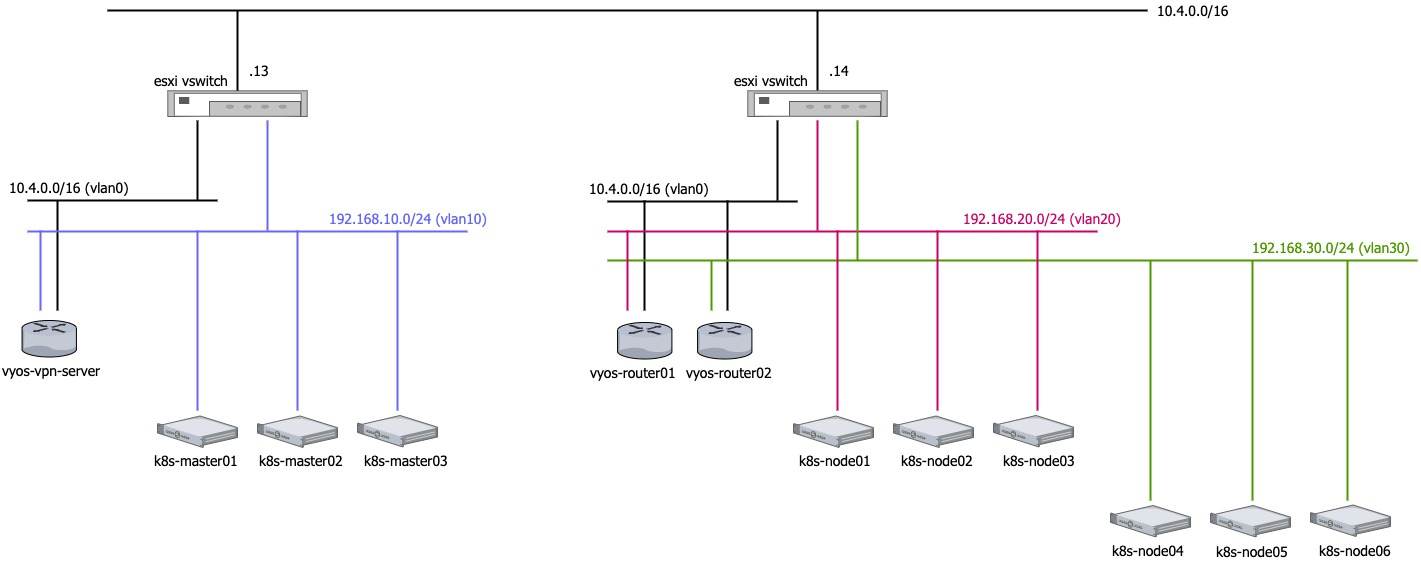
\includegraphics[width=\textwidth]{./figures/network-diagram.jpg}
    \caption{ネットワーク構成図}
  \end{center}
\end{figure}

%%% Local Variables:
%%% mode: japanese-latex
%%% TeX-master: "../bthesis"
%%% End:
